% Paquets généraux
\documentclass[a4paper,12pt,titlepage]{article}
\usepackage[T1]{fontenc}
\usepackage[utf8]{inputenc}
\usepackage[french]{babel}
\usepackage[gen]{eurosym}
%\usepackage[dvips]{graphicx}
\usepackage{fancyhdr}
\usepackage{pdfpages} 
\usepackage{multido}
\usepackage{hyperref}
%\usepackage{textcomp}
%\usepackage{aeguill}
\usepackage{schemabloc}
\usepackage[bitstream-charter]{mathdesign}
\usepackage{pstricks}
\usepackage{helvet}

\newcommand{\id}{54}
\newcommand{\nom}{Liaisons mécaniques}
\newcommand{\sequence}{04}
\newcommand{\num}{01}
\newcommand{\type}{TP}
\newcommand{\descrip}{Modélisation d'un solide. Comportement des liaisons mécaniques. Modéliser les mécanismes du laboratoire par un schéma cinématique, paramétré.}
\newcommand{\competences}{A3-C4: Analyse d'architecture et de comportement \\ &  Mod1-C1: Isolement d'un solide ou d'un système de solides \\ &  Mod2-C10-1: Modèle de solide indéformable \\ &  Mod2-C11: Modélisation géométrique et cinématique des mouvements entre solides indéformables \\ &  Mod2-C12: Modélisation cinématique des liaisons entre solides \\ &  Mod2-C15: Modélisation des actions mécaniques \\ &  Rés-C6: Utilisation d'un solveur ou d'un logiciel multi physique \\ &  Com1-C1: Différents descripteurs introduits dans le programme \\ &  Com2-C4: Outils de communication}
\newcommand{\nbcomp}{9}
\newcommand{\systemes}{Plateforme Stewart}
\newcommand{\systemessansaccent}{Plateforme Stewart}
\newcommand{\ilot}{2}
\newcommand{\ilotstr}{02}
\newcommand{\dossierilot}{\detokenize{Ilot_02 Plateforme Stewart}}
\newcommand{\imageun}{Plateforme}

\newcommand{\urlsysteme}{\href{https://www.costadoat.fr/systeme/57}{Ressources système}}
\newcommand{\matlabsimscape}{\href{https://github.com/Costadoat/Sciences-Ingenieur/raw/master/Systemes/Plateforme Stewart/Plateforme_Stewart_Simscape.zip}{Modèle Simscape}}
\newcommand{\solidworks}{\href{https://github.com/Costadoat/Sciences-Ingenieur/raw/master/Systemes/Plateforme Stewart/Plateforme_Stewart_Solidworks.zip}{Modèle Solidworks}}
\newcommand{\edrawings}{\href{https://github.com/Costadoat/Sciences-Ingenieur/raw/master/Systemes/Plateforme Stewart/Plateforme_Stewart.EASM}{Modèle eDrawings}}
\newcommand{\test}{Stewart_param1}
\newcommand{\testi}{Stewart_param2}
\newcommand{\testii}{Stewart_param3}
\newcommand{\testiii}{Stewart_param4}
\newcommand{\testiiii}{Stewart_euler}

\newcommand{\auteurun}{Renaud Costadoat}
\newcommand{\institute}{Lycée Dorian}


\usepackage{color}
\usepackage{xcolor}
\usepackage{colortbl}
\usepackage{helvet}
\renewcommand{\familydefault}{\sfdefault}
\usepackage{amsfonts}
\usepackage{amsmath}
%\usepackage{xspace}
\usepackage{varioref}
\usepackage{tabularx}
%\usepackage{floatflt}
\usepackage{graphics}
\usepackage{wrapfig}
\usepackage{textcomp}
\usepackage{tikz}
\usepackage{wrapfig}
\usepackage{gensymb}
\usepackage[european]{circuitikz}
\usetikzlibrary{babel}
\usepackage{ifthen}
\usepackage{cancel}
\usepackage{etoolbox}
\usepackage{multirow}
%\usepackage{boxedminipage}
\definecolor{gris25}{gray}{0.75}
\definecolor{bleu}{RGB}{18,33,98}
\definecolor{bleuf}{RGB}{42,94,171}
\definecolor{bleuc}{RGB}{231,239,247}
\definecolor{rougef}{RGB}{185,18,27}
\definecolor{rougec}{RGB}{255,188,204}%255,230,231
\definecolor{vertf}{RGB}{103,126,82}
\definecolor{vertc}{RGB}{220,255,191}
\definecolor{forestgreen}{rgb}{0.13,0.54,0.13}
\definecolor{blcr}{rgb}{0.59,0.69,0.84}
\definecolor{blfr}{rgb}{0.32,0.51,0.75}
\definecolor{orfr}{rgb}{0.90,0.42,0.15}
\definecolor{orcr}{rgb}{0.90,0.65,0.50}
\definecolor{orangef}{rgb}{0.659,0.269,0.072}
\definecolor{orange}{rgb}{0.58,0.35,0.063}
\definecolor{orangec}{rgb}{0.43,0.32,0.25}
\definecolor{rcorrect}{rgb}{0.6,0,0}
\definecolor{sequence}{rgb}{0.75,0.75,0.75}
\definecolor{competences}{rgb}{0.61,0.73,0.35}
\definecolor{grisf}{HTML}{222222}
\definecolor{grisc}{HTML}{636363}
\definecolor{normal}{HTML}{4087c4}
\definecolor{info}{HTML}{5bc0de}
\definecolor{success}{RGB}{92,184,92}
\definecolor{warning}{RGB}{240,173,78}
\definecolor{danger}{RGB}{217,83,79}
\hypersetup{                    % parametrage des hyperliens
    colorlinks=true,                % colorise les liens
    breaklinks=true,                % permet les retours à la ligne pour les liens trop longs
    urlcolor= blfr,                 % couleur des hyperliens
    linkcolor= orange,                % couleur des liens internes aux documents (index, figures, tableaux, equations,...)
    citecolor= forestgreen                % couleur des liens vers les references bibliographiques
    }

% Mise en page
\pagestyle{fancy}

\setlength{\hoffset}{-18pt}

\setlength{\oddsidemargin}{0pt} 	% Marge gauche sur pages impaire2s
\setlength{\evensidemargin}{0pt} 	% Marge gauche sur pages paires
\setlength{\marginparwidth}{00pt} 	% Largeur de note dans la marge
\setlength{\headwidth}{481pt} 	 	% Largeur de la zone de tête (17cm)
\setlength{\textwidth}{481pt} 	 	% Largeu\textbf{r de la zone de texte (17cm)
\setlength{\voffset}{-18pt} 		% Bon pour DOS
\setlength{\marginparsep}{7pt}	 	% Séparation de la marge
\setlength{\topmargin}{-30pt} 		% Pas de marge en haut
\setlength{\headheight}{55pt} 		% Haut de page
\setlength{\headsep}{20pt} 		% Entre le haut de page et le texte
\setlength{\footskip}{30pt} 		% Bas de\textbf{ page + séparation
\setlength{\textheight}{700pt} 		% Hauteur de l'icone zone de texte (25cm)
\setlength\fboxrule{1 pt}
\renewcommand{\baselinestretch}{1}
\setcounter{tocdepth}{1}
\newcommand{\cadre}[2]
{\fbox{
  \begin{minipage}{#1\linewidth}
   \begin{center}
    #2\\
   \end{center}
  \end{minipage}
 }
}

\newcommand{\reponse}[1][4]
{
\multido{}{#1}
{\begin{center}\makebox[0.9\linewidth]{}  \\
\begin{center}\makebox[0.9\linewidth]{\dotfill} \\ \end{center}
}}

\newcommand{\titre}[1]
{\begin{center}
\cadre{0.8}{\huge #1} 
\end{center}
}


% En tête et pied de page
\lhead{\nom}
\rhead{
\includegraphics[width=2cm]{../../img/logo}}
\lfoot{Renaud Costadoat}
\cfoot{Page \thepage}

\fancypagestyle{correction}{%
  \fancyhf{}
  \lhead{\colorbox{danger}{\begin{minipage}{0.65\paperwidth} \textcolor{white}{\textbf{Correction}} \end{minipage}} }
  \rhead{
\includegraphics[width=2cm]{../../img/logo}}
  \lfoot{Renaud Costadoat}
  \rfoot{\colorbox{danger}{\begin{minipage}{0.6\paperwidth} \begin{flushright}\textcolor{white}{\textbf{Correction}}\end{flushright} \end{minipage}} }}

\renewcommand{\footrulewidth}{0.4pt}

\usepackage{eso-pic}
\newcommand{\BackgroundPic}{%
\put(0,0){%
\parbox[b][\paperheight]{\paperwidth}{%
\vfill
\begin{center}
\hspace{0.5cm}\vspace{0.5cm}

\includegraphics[width=\paperwidth,height=\paperheight,%
keepaspectratio]{../../img/fond3}%
\end{center}
\vfill
}}}

\newcommand{\BackgroundPicdeux}{%
\put(25,-30){%
\parbox[b][\paperheight]{\paperwidth}{%
\vfill
\begin{center}
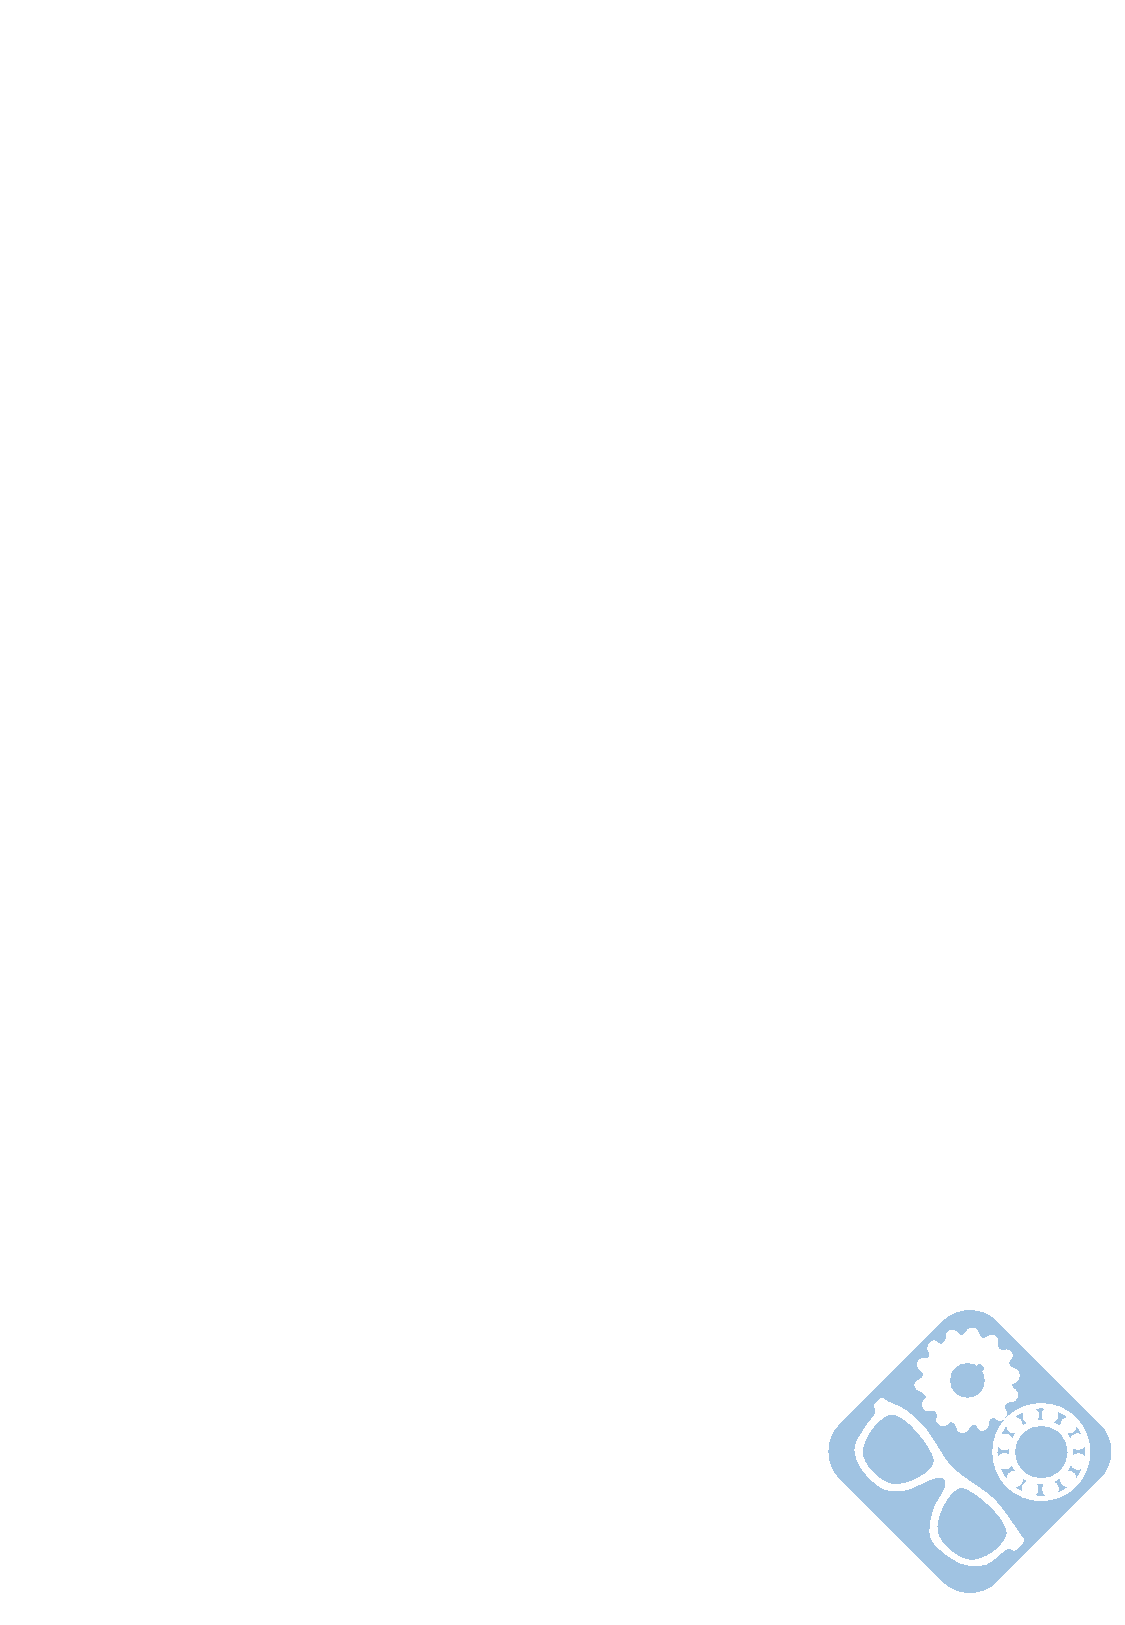
\includegraphics[width=\paperwidth,height=\paperheight,%
keepaspectratio]{../../img/fond4}%
\end{center}
\vfill
}}}

\begin{document}

\AddToShipoutPicture{\BackgroundPicdeux}

\pagestyle{fancy}

\section{La moto trial}

\begin{figure}[!h]
\begin{minipage}{0.4\linewidth}
Le trial est une discipline sportive à moto (figure \ref{img1}), à vélo (voire en vélo monocycle), en automobile ou en camion. Le trial consiste, en effet, à franchir des obstacles naturels ou artificiels.

Le temps n'est pas pris en compte dans ces compétitions, par contre, il est interdit aux compétiteurs de poser le pied à terre. C'est pour cela qu'à tout instant, il doivent tant que faire se peut conserver leur équilibre statique.
\end{minipage}
\hfill
\begin{minipage}{0.5\linewidth}
 \begin{center}
 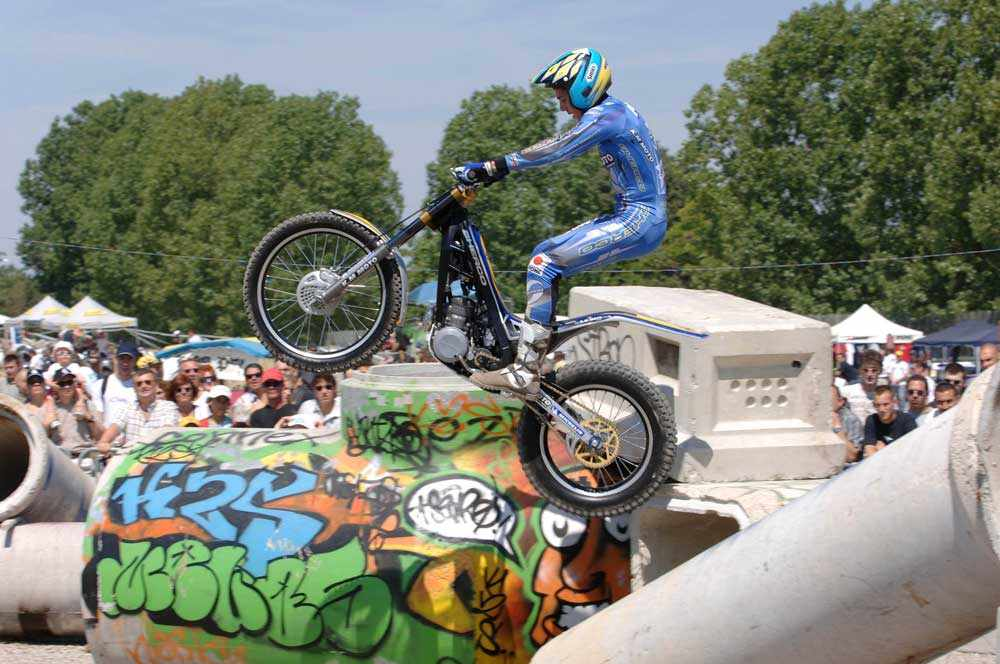
\includegraphics[width=0.7\linewidth]{img/Trial.jpg}
 \end{center}
 \caption{Compétiteur de moto trial}
 \label{img1}
 \end{minipage}
\end{figure}

\begin{figure}[!h]
\begin{minipage}{0.48\linewidth}
 \centering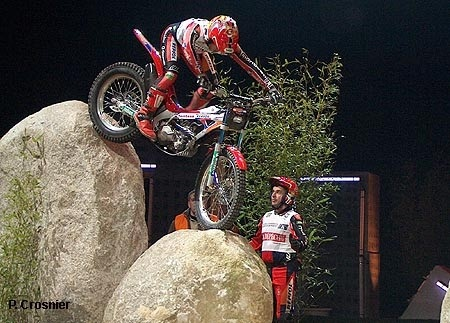
\includegraphics[width=0.7\linewidth]{img/Trial_des.jpg}
 \caption{Moto en phase de descente}
  \label{img2}
\end{minipage}
\hfill
\begin{minipage}{0.48\linewidth}
 La figure \ref{img2} montre un compétiteur en phase de descente d'un bloc. Les paramètres sont les suivants:
 \begin{itemize}
  \item Soit $A$ le point de contact de la roue arrière (pente 45\%),
  \item Soit $B$ le point de contact de la roue avant (pente 0\%),
  \item $\overrightarrow{AB}=1,9.\overrightarrow{x_0}$ (en mètre),
  \item Le motard et la moto seront considérés dans le plan $(\overrightarrow{x_0},\overrightarrow{y_0})$,
  \item Le centre de gravité $G$ de l'ensemble moto et motard est défini tel que :
  
  $\overrightarrow{AG}=0,8.\overrightarrow{x_0}+0,7.\overrightarrow{y_0}$ (en mètre).
  \item La masse de l'ensemble moto plus moteur est de 280 kilogrammes,
  \item $(\overrightarrow{x_0},\overrightarrow{x})=45°$
 \end{itemize}
\end{minipage}
\end{figure}

\paragraph{Question 1:} Effectuer une représentation plane du problème.

\paragraph{Question 2:} Déterminer les actions mécaniques exercées sur l'ensemble moto et motard (des frottements ne seront appliqués qu'au point A.

\paragraph{Question 3:} En déduire le coefficient de frottement nécessaire pour maintenir la moto.

\paragraph{Question 4:} Déterminer les actions mécaniques exercées sur l'ensemble moto et motard (des frottements ne seront appliqués qu'au point B.

\paragraph{Question 5:} En déduire le coefficient de frottement nécessaire pour maintenir la moto.

\paragraph{Question 6:} D'après vous, le freinage sur quelle roue sera le plus efficace?


\newpage

~\

\newpage

\section{Avion militaire}

\begin{minipage}{0.4\linewidth}
 \centering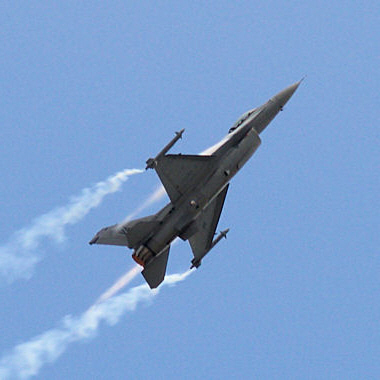
\includegraphics[width=0.7\linewidth]{img/avion_chasse.jpg}
\end{minipage}
\hfill
\begin{minipage}{0.56\linewidth}
Un avion militaire est en phase ascentionnelle à vitesse constante suivant un angle de 15º sous la poussée $\overrightarrow{F}$ (12 000 daN) des réacteurs. $\overrightarrow{R}$ schématise l'action de la resistance de l'air sur l'ensemble de la structure, $\overrightarrow{S}$ est la résultante des actions de sustentation sur les ailes et $\overrightarrow{A}$ schématise la résultante des actions stabilisatrices de l'air sur l'aileron arrière. $\overrightarrow{P}$ (30 000 daN) est le poids de l'appareil.
\end{minipage}

\begin{center}
 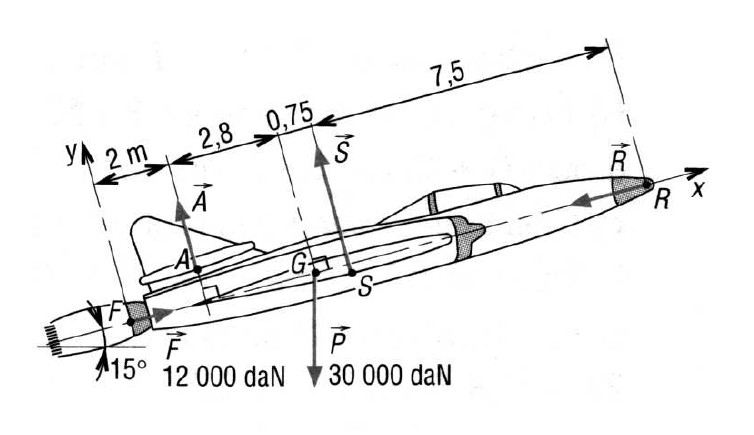
\includegraphics[width=0.9\linewidth]{img/avion_schem.jpg}
\end{center}

\paragraph{Question 1:} Déterminer $\overrightarrow{A}$, $\overrightarrow{S}$ et $\overrightarrow{R}$ si toutes les actions sont supposées contenues dans le plan de symétrie de l'appareil.


\newpage

~\

\newpage

\section{Serrage de pièce}

\begin{minipage}{0.4\linewidth}
 \centering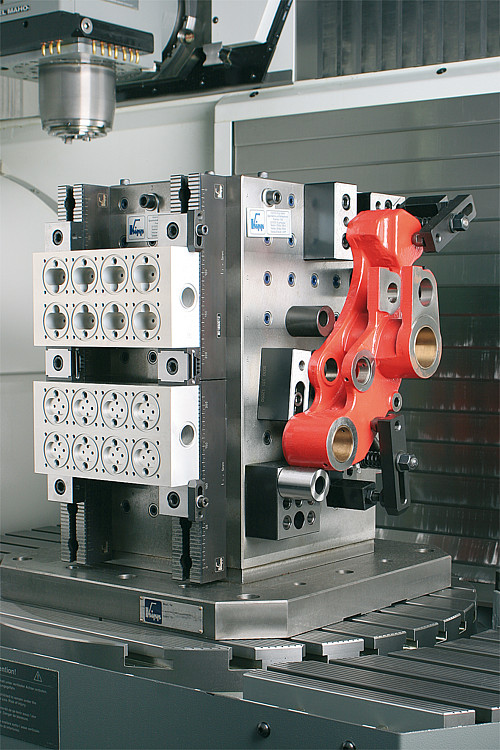
\includegraphics[width=0.7\linewidth]{img/KMSS.jpg}
\end{minipage}
\hfill
\begin{minipage}{0.56\linewidth}
Le dispositif proposé fait partie d'un montage d'usinage. La pièce à usiner (4) est bridée en B par un renvoie (3) articulé (liaison pivot) en C sur la bâti (1) du montage. Le serrage de la pièce est réalisé par une vis de pression (2) agissant en 1 (contact ponctuel). Les poids des pièces sont négligés, $\overrightarrow{A_{2 \rightarrow 3}}$ (300 daN) schématise l'action de la vis sur le renvoi, l'action du ressort est négligée.
\end{minipage}

\begin{center}
 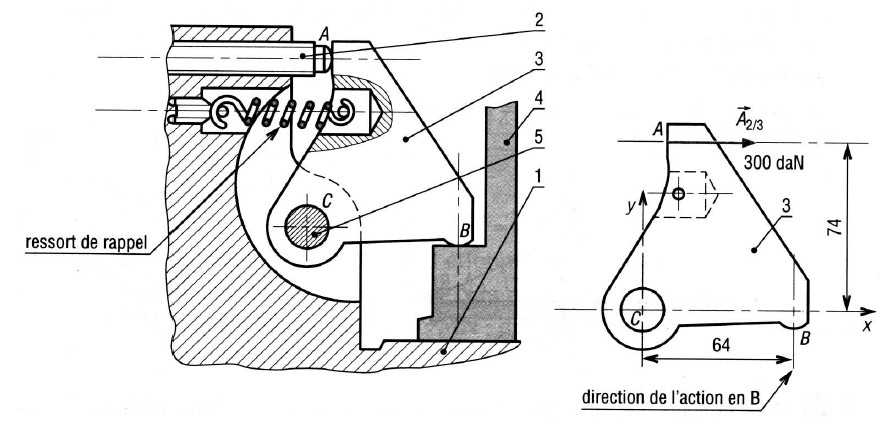
\includegraphics[width=0.9\linewidth]{img/Bride.jpg}
\end{center}

\paragraph{Question 1:} Déterminer les actions exercées en B et C.

\newpage

~\

\newpage

\section{Porte tôle}

\begin{minipage}{0.4\linewidth}
 \centering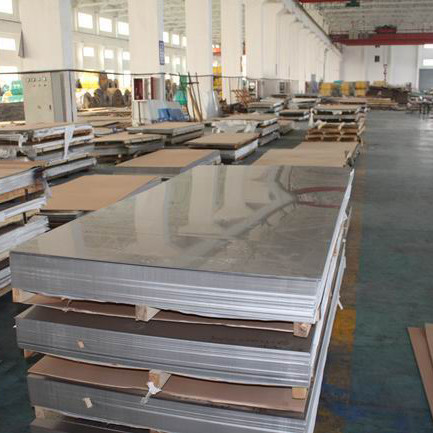
\includegraphics[width=0.7\linewidth]{img/tole_hor.jpg}
\end{minipage}
\hfill
\begin{minipage}{0.56\linewidth}
De part leur géométrie, la manipulation des tôles est souvent complexe. En général, elles sont transportées horizontalement. Cependant, cela ne peut pas être le cas pour une tôle seule, en effet, celle-ci fléchirait sous son propre poids, c'est pourquoi elles sont dans ce cas transportées verticalement. Le problème consiste alors à trouver un moyen de les fixer au système qui va les déplacer. Le porte-tôle étudié est composé de deux molettes en liaison pivot d'axe $(B,\overrightarrow{z})$ avec les flasques. Elles serrent la tôle sous l'action de deux biellettes articulées en C et C' avec les molettes et en D et D' avec l'étrier auquel est accroché le câble.
\end{minipage}

\begin{center}
 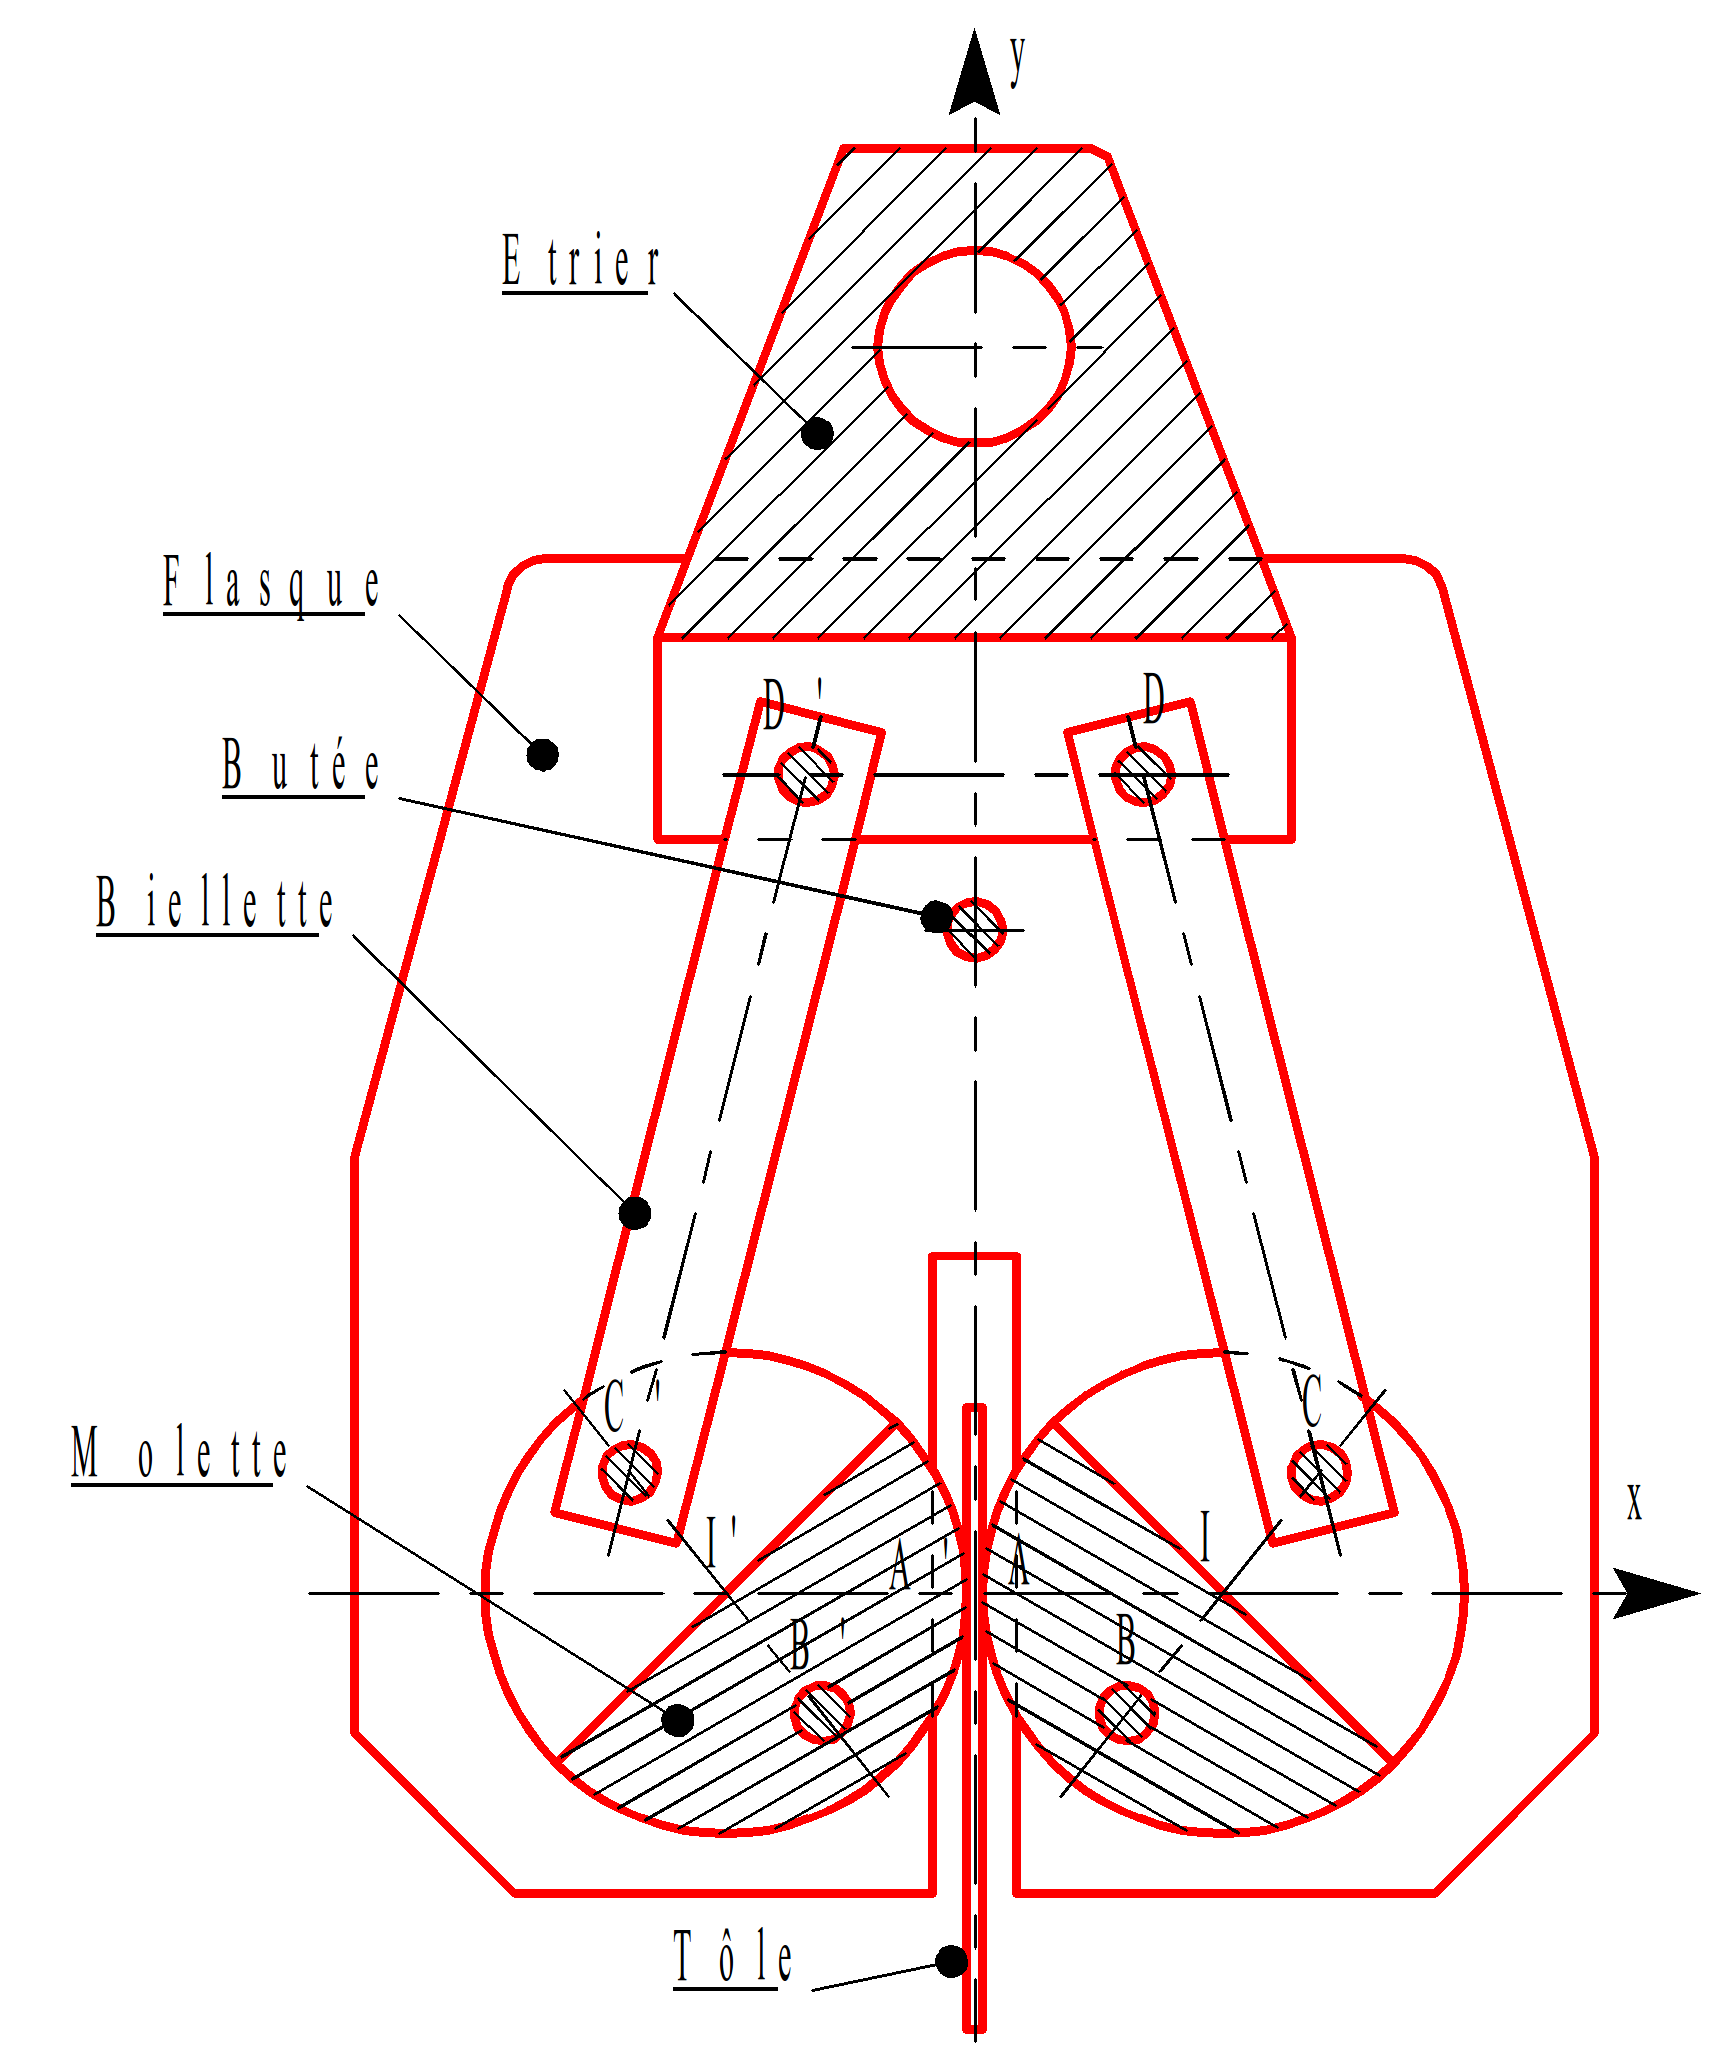
\includegraphics[width=0.6\linewidth]{img/porte_tole.png}
\end{center}

Toutes les liaisons sont sans frottement sauf la liaison entre la tôle et les molettes et que la masse des pièces est négligeable devant la masse de la tôle. Les dimensions sont (en millimètres):
\begin{itemize}
 \item $\overrightarrow{IA}=-30.\overrightarrow{x}$,
 \item $\overrightarrow{IC}=-\overrightarrow{IB}=12.\overrightarrow{x}+15.\overrightarrow{y}$,
 \item $\overrightarrow{ID}=-10.\overrightarrow{x}+102.\overrightarrow{y}$.
\end{itemize}

\paragraph{Question 1:} Déterminer la valeur minimale du coefficient de frottement entre la tôle et les molettes pour que ce dispositif fonctionne.

\newpage

~\

\end{document}